\documentclass[10pt]{beamer}

\usepackage[T2A]{fontenc}
\usepackage[utf8]{inputenc}
\usepackage[russian]{babel}
\usepackage{multicol}
\usepackage{hyperref}
\usepackage{caption}
\usepackage{subcaption}
\setbeamertemplate{navigation symbols}{} %отключение значков
\setbeamertemplate{caption}[numbered]
\usetheme{Warsaw}
\setbeamertemplate{footline}{%
    \hspace{0.94\paperwidth}%
    \usebeamerfont{title in head/foot}%
    \insertframenumber\,/\,\inserttotalframenumber%
}
\newcommand{\pdiff}[2]{\frac{\partial #1}{\partial #2}}
\newcommand{\op}[1]{\mathop{\mathrm{#1}}}
\graphicspath{{pictures/}}
\begin{document}

\title{Программный генератор сигналов на основе микроконтроллера STM32}
\author{Студент гр. 506: Вебер Данил Сергеевич\\Руководитель:  ст.пр. Уланов Пётр Николаевич}
\date{2024}
\institute{Алтайский государственный университет}


\frame{\titlepage}

\begin{frame}{Актуальность}
  
  \begin{figure}
  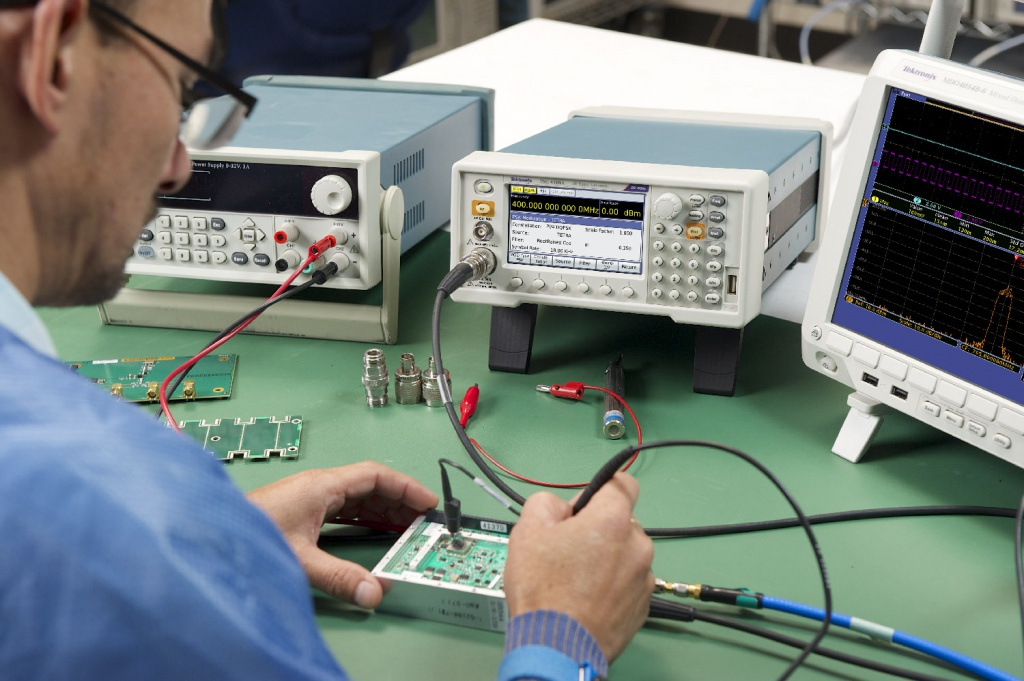
\includegraphics[width=0.85\textwidth]{actual2}
  \caption*{Тестирование и отладка устройства.}
  \end{figure}
\end{frame}

\begin{frame}{Цель и задачи}
  \textbf{Цель:} разработка программного генератора сигналов на микроконтроллере.

  \textbf{Задачи:} 
	\begin{enumerate}
		\item Исследовать методы генерации сигналов и осуществить выбор;
		\item Рассмотреть семейства микроконтроллеров и осуществить выбор;
		\item Выбрать среду разработки;
		\item Разработать программу;
		\item Спроектировать устройство;
		\item Протестировать генератор.
	\end{enumerate}
\end{frame}

\begin{frame}{Методы цифровой генерации сигнала}
  \begin{enumerate}
		\item Метод аппроксимации. 
		
		+: Малый объем памяти, так как хранятся только параметры сигнала. 
		
		---: Высокие вычислительные затраты, что ограничивает максимальную частоту сигнала.
		
		\item CORDIC.
		
		+: Быстродействие и высокая точность системы, благодаря итерационному методу.
		
		---: Сложность алгоритма и потребность в специализированных вычислениях.
		
		\item Табличный метод.
		
		+: Возможность генерации сигналов с более высокой частотой из-за отсутствия вычислений.
		
		---: Необходимость хранения больших объёмов данных в памяти.
		
		\item Метод DDS.
		
		+: Гибкость, простота реализации и высокая точность регулирования частоты.
		
		---: Потребность в дополнительных вычислениях для генерации сигнала.
  \end{enumerate}
\end{frame}

\begin{frame}
\frametitle{Метод DDS}
\begin{columns}
\begin{column}{0.55\textwidth}
  	Для адресации используется аккумулятор фазы и код частоты. 
\vspace{0.25cm}

	Старшая часть аккумулятора фазы отвечает за адресацию ячейки в таблице отсчётов, а младшая за шаг в этой таблице. Размером же шага является код частоты.

\vspace{0.25cm}
	Аккум. фазы + Код частоты = Адрес отсчёта 
	
	0x0000 + 0x0100 = 0x0100

	0x0000 + 0x0200 = 0x0200
	
	0x0000 + 0x0080 + 0x0080 = 0x0100
\end{column}
\begin{column}{0.45\textwidth}  
    \begin{center}
    \begin{figure}
    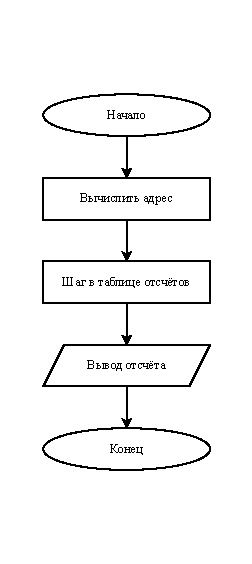
\includegraphics[width=0.6\textwidth]{dds_block}
     \caption*{Алгоритм метода DDS.}
    \end{figure}
     \end{center}
\end{column}
\end{columns}
\end{frame}

\begin{frame}{Существующие генераторы}
\begin{figure}
     \begin{subfigure}[H]{0.35\textwidth}
         \centering
         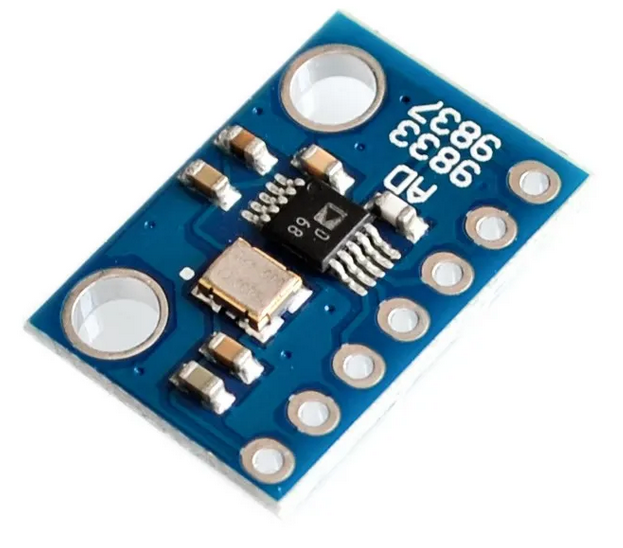
\includegraphics[width=\textwidth]{ad9833}
         \caption*{Модуль AD9833.}
     \end{subfigure}
     \hfill
     \begin{subfigure}[H]{0.5\textwidth}
         \centering
         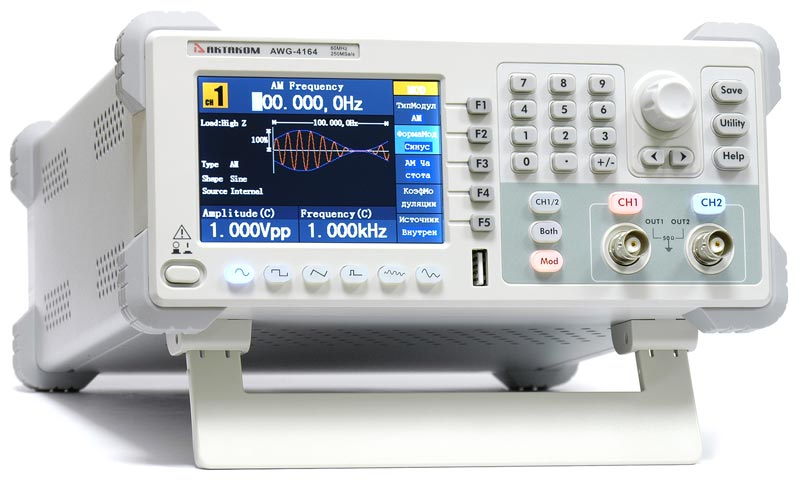
\includegraphics[width=\textwidth]{AWG-4112}
         \caption*{АКТАКОМ AWG-4112.}
     \end{subfigure}
        %\caption*{Генераторы сигналов.}
\end{figure}
\begin{columns}
\begin{column}{0.5\textwidth}
\vspace{0.3cm}

+: компактность, возможность интеграции с другими компонентами.

---: необходимость в управляющем устройстве.
\end{column}
\begin{column}{0.5\textwidth}  
+: высокая точность, широкий диапазон частот.

---: большие размеры, высокая стоимость.
\end{column}
\end{columns}
\end{frame}

\begin{frame}{Микроконтроллеры}
\begin{small}
\begin{table}[H]
\caption*{Параметры микроконтроллеров}
\begin{tabular}{|p{1.5 cm}|p{1.9 cm}|p{1.9 cm}|p{1.9 cm}|p{1.9 cm}|}
\hline
        Параметр & ATtiny10 & ATmega32 & STM32L010F4 & STM32F103xC \\ \hline
        Частота & 20 МГц & 20 МГц & 32 МГц & 72 МГц \\ \hline
        FLASH & 1 Кбайт & 32 Кбайт & 16 Кбайт & 256 Кбайт \\ \hline
        RAM & 64 байт & 2 Кбайт & 2 Кбайт & 48 Кбайт \\ \hline
        SPI & - & + & + & + \\ \hline
        I2C & - & +	 & + & + \\ \hline
        Питание & 1,8 --- 5,5 В & 1,8 --- 5,5 В & 1,8 --- 3,6 В & 1,8 --- 3,6 В \\ \hline
\end{tabular}
\end{table}
\end{small}
\end{frame}

\begin{frame}{Выбор микроконтроллера и среды разработки}
\begin{figure}
     \begin{subfigure}[H]{0.4\textwidth}
         \centering
         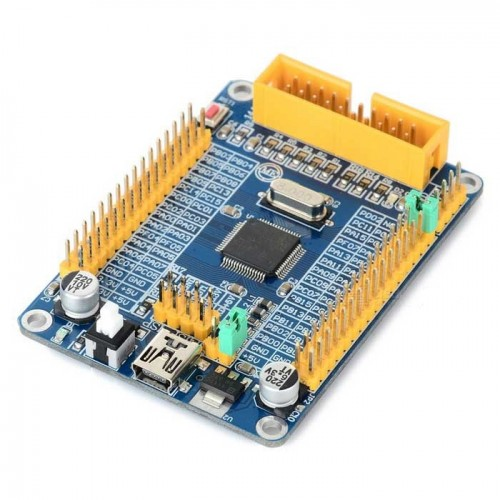
\includegraphics[width=\textwidth]{stmka}
         \caption*{Микроконтроллер}
     \end{subfigure}
     \hfill
     \begin{subfigure}[H]{0.35\textwidth}
         \centering
         
\includegraphics[width=\textwidth]{PlatformIO}
         \caption*{IDE}
     \end{subfigure}
        %\caption*{Инструменты.}
\end{figure}
  Микроконтроллер: STM32F103RCT6 на отладочной плате.
  
  Среда разработки: VSCode + PlatformIO.
  
  Язык программирования: C.
  
  Библиотека: libopencm3.
\end{frame}


\begin{frame}{Программа для генерации сигналов}
  \begin{figure}
  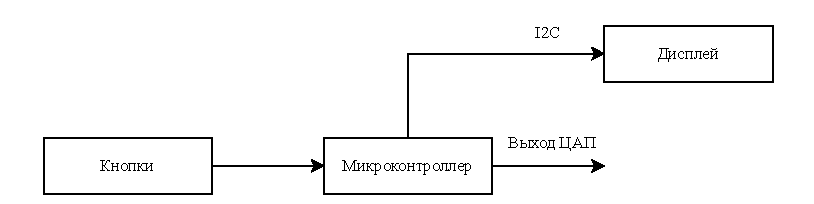
\includegraphics[width=1\textwidth]{struct_gen}
  \caption*{Структурная схема генератора сигналов.}
  \end{figure}
  Программа должна выполнять три действия:
  	\begin{enumerate}
		\item Вывод отсчёта в ЦАП;
		\item Обработка кнопок;
		\item Вывод информации на дисплей.
	\end{enumerate}
\end{frame}

\begin{frame}{Программа для генерации сигналов}
  \begin{figure}
  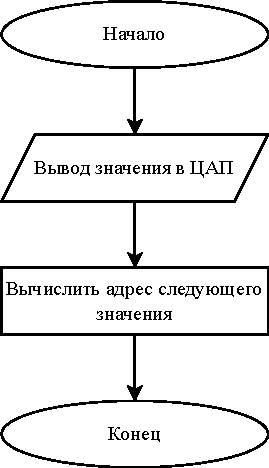
\includegraphics[width=0.4\textwidth]{dac}
  \caption*{Блок-схема алгоритма вывода отсчёта в ЦАП (прерывание таймера 2).}
  \end{figure}
\end{frame}

\begin{frame}{Программа для генерации сигналов}
  \begin{figure}
  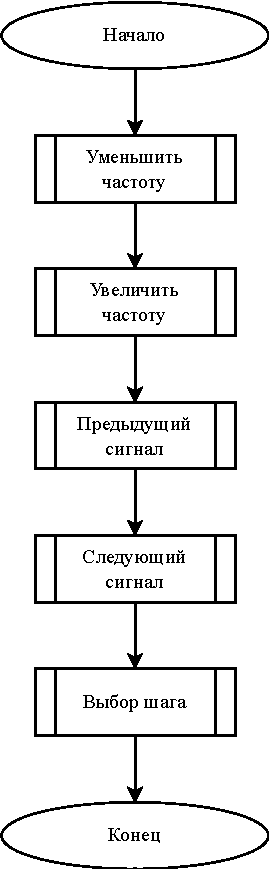
\includegraphics[width=0.23\textwidth]{buttons}
  \caption*{Блок-схема алгоритма обработки кнопок (прерывание таймера 3).}
  \end{figure}
\end{frame}

\begin{frame}{Программа для генерации сигналов}
  \begin{figure}
  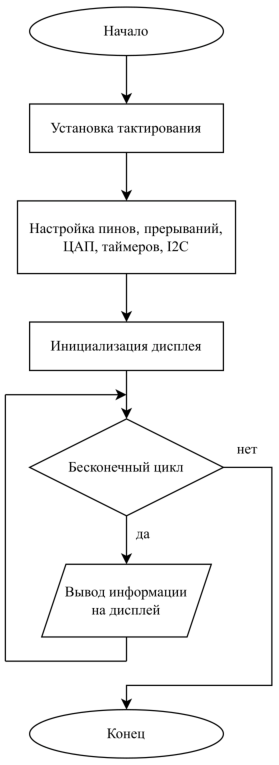
\includegraphics[width=0.275\textwidth]{main}
  \caption*{Блок-схема алгоритма главной функции.}
  \end{figure}
\end{frame}

\begin{frame}{Проектирование генератора сигналов}
  \begin{figure}
  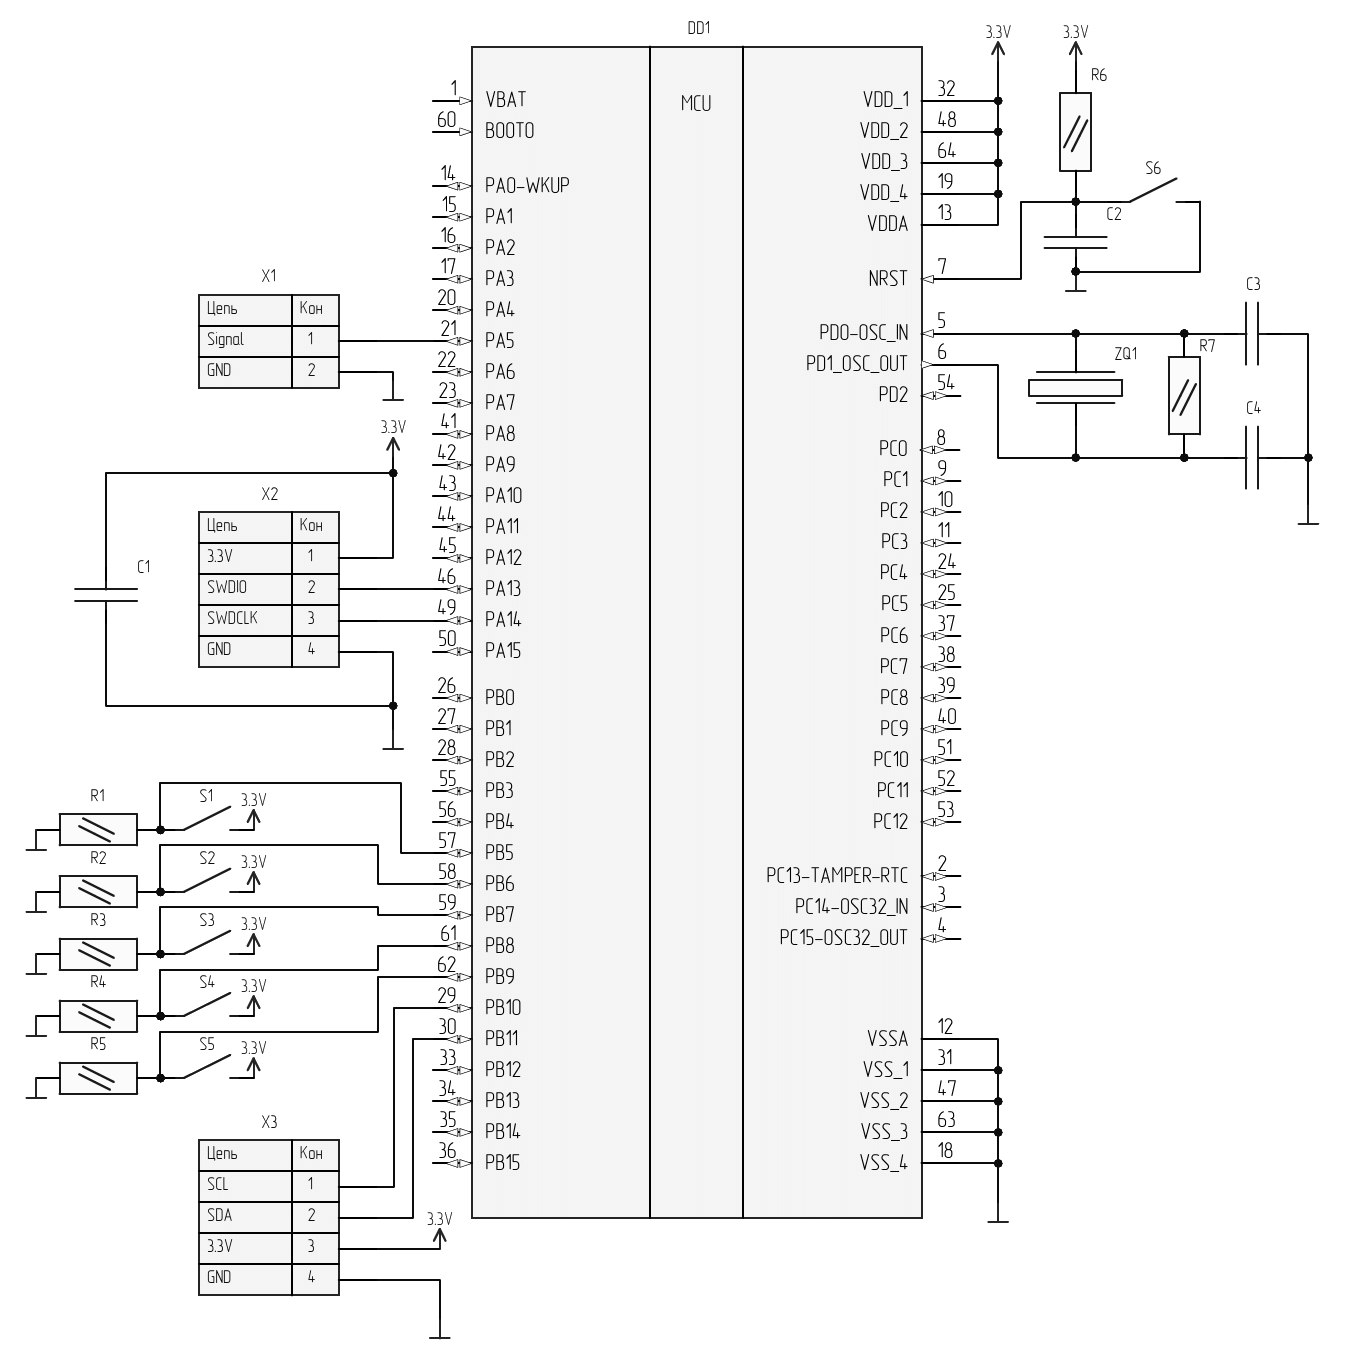
\includegraphics[width=0.75\textwidth]{scheme-cropped}
  \caption*{Фрагмент схемы электрической принципиальной.}
  \end{figure}
\end{frame}

\begin{frame}{Проектирование генератора сигналов}
\begin{figure}
     \begin{subfigure}[H]{0.45\textwidth}
         \centering
         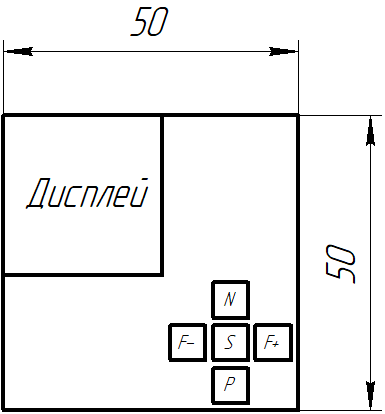
\includegraphics[width=\textwidth]{func_gen}
         \caption*{Схема расположения периферии.}
     \end{subfigure}
     \hfill
     \begin{subfigure}[H]{0.5\textwidth}
         \centering
         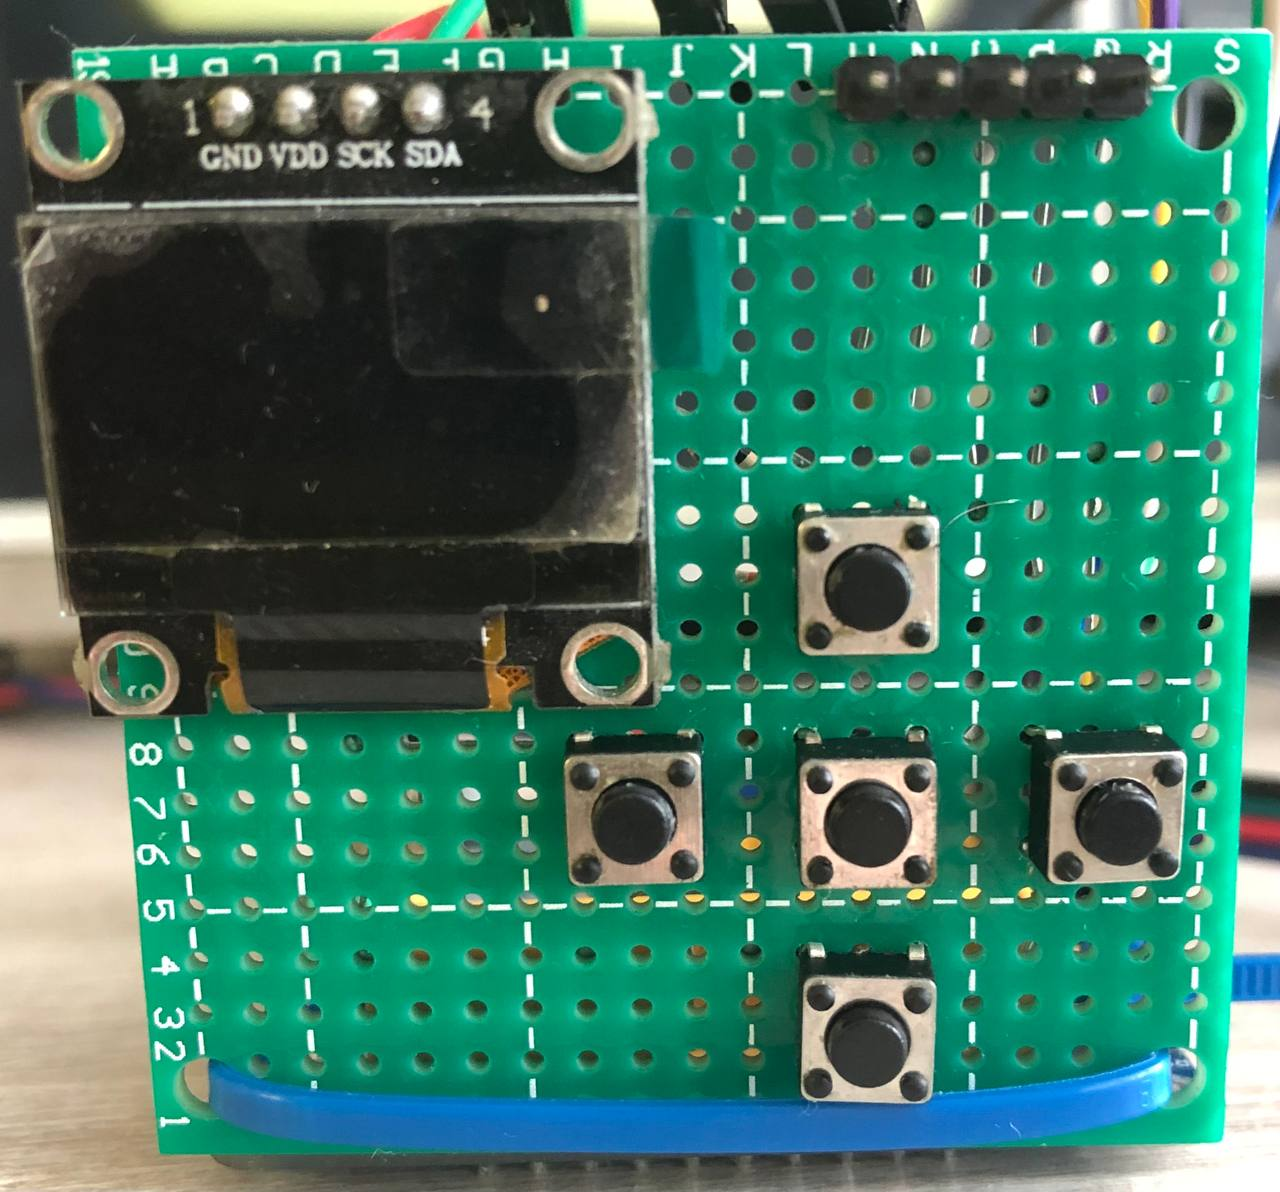
\includegraphics[width=\textwidth]{m1}
         \caption*{Полученная плата периферии.}
     \end{subfigure}
        %\caption*{Конструирование платы периферии.}
\end{figure}
\end{frame}

\begin{frame}{Проектирование генератора сигналов}
  \begin{figure}
  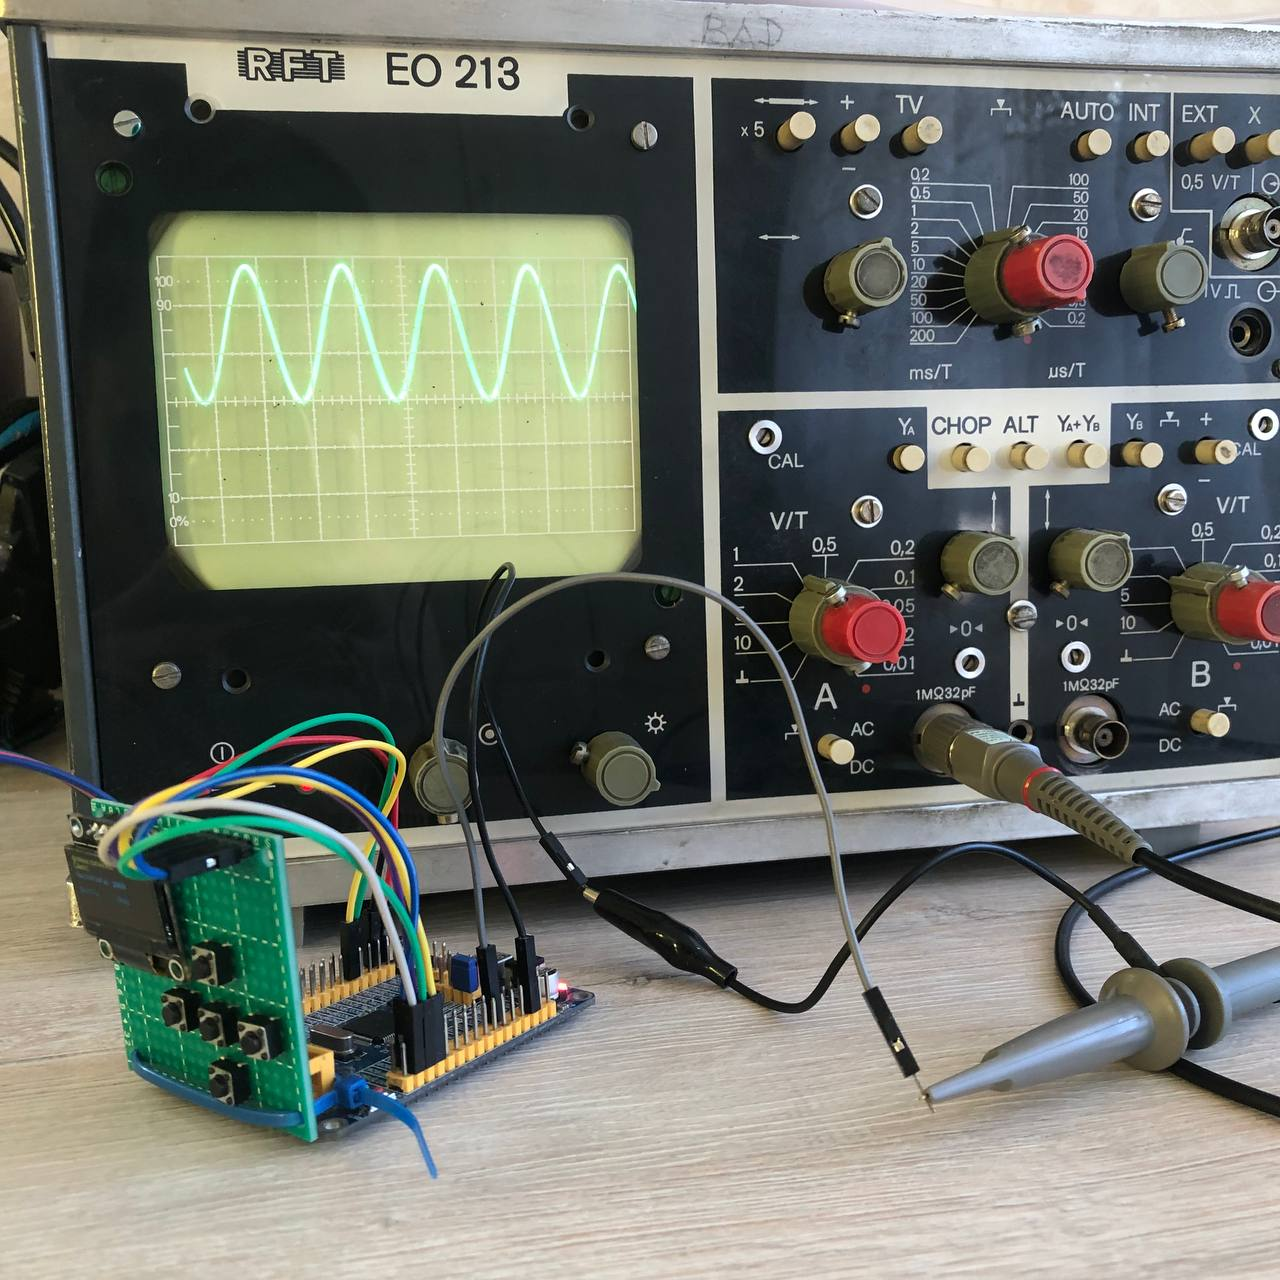
\includegraphics[width=0.75\textwidth]{m2}
  \caption*{Макет устройства.}
  \end{figure}
\end{frame}

\begin{frame}{Тестирование}
\begin{figure}
     \begin{subfigure}[H]{0.45\textwidth}
         \centering
         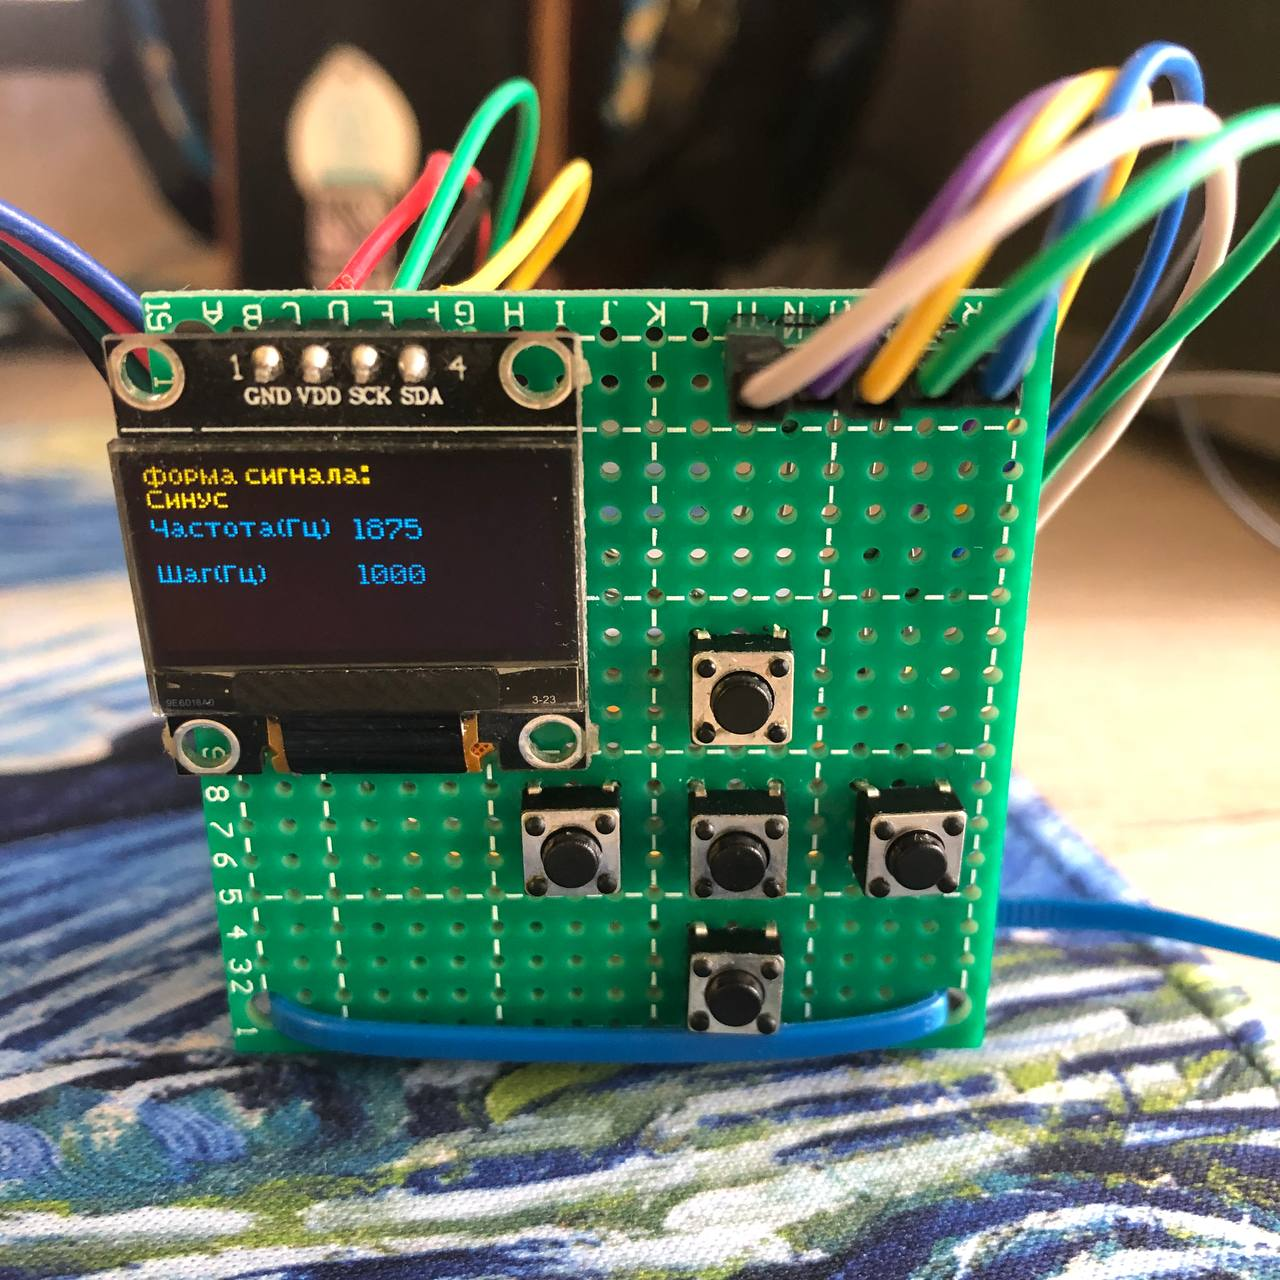
\includegraphics[width=\textwidth]{test4_u_f}
         \caption*{Состояние устройства.}
     \end{subfigure}
     \hfill
     \begin{subfigure}[H]{0.45\textwidth}
         \centering
         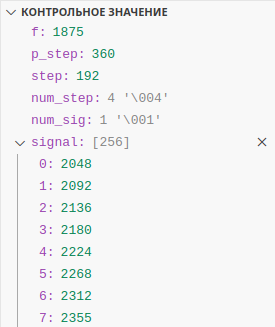
\includegraphics[width=\textwidth]{test4_o_f}
         \caption*{Состояние в отладчике.}
     \end{subfigure}
        %\caption*{Работа устройства.}
\end{figure}
\end{frame}

\begin{frame}{Тестирование}
  \begin{figure}
  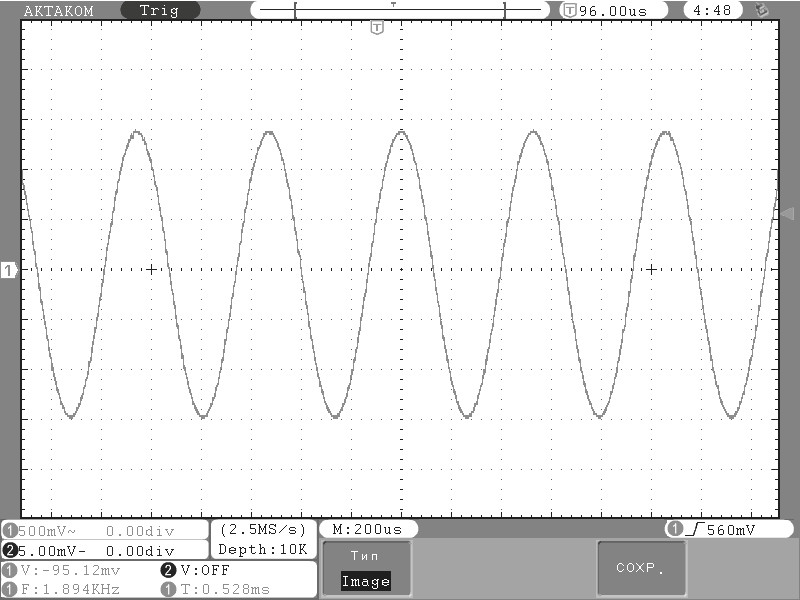
\includegraphics[width=1\textwidth]{1875}
  \caption*{Синусоидальный сигнал с частотой 1875 Гц.}
  \end{figure}
\end{frame}

\begin{frame}{Тестирование}
\begin{figure}
     \begin{subfigure}[H]{0.4\textwidth}
         \centering
         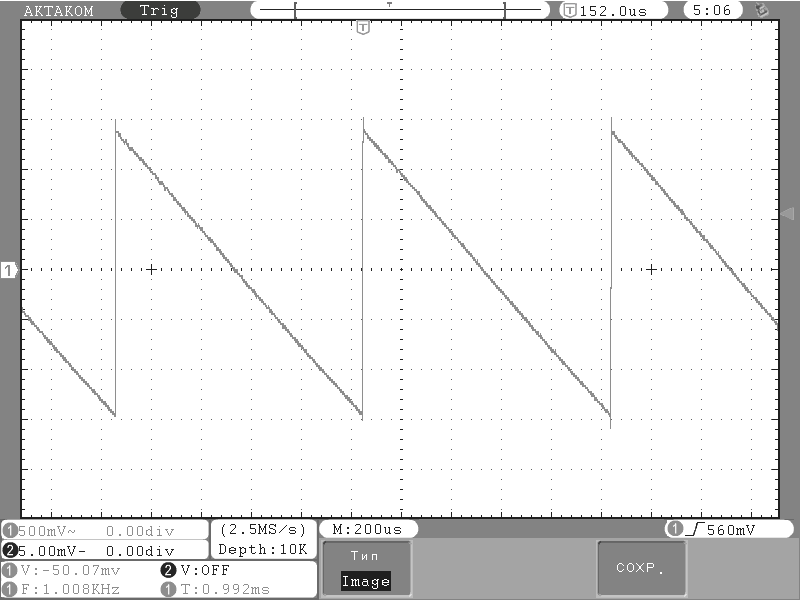
\includegraphics[width=\textwidth]{l_saw1}
         \caption*{Обратная пилообразная}
     \end{subfigure}
     \hfill
     \begin{subfigure}[H]{0.4\textwidth}
         \centering
         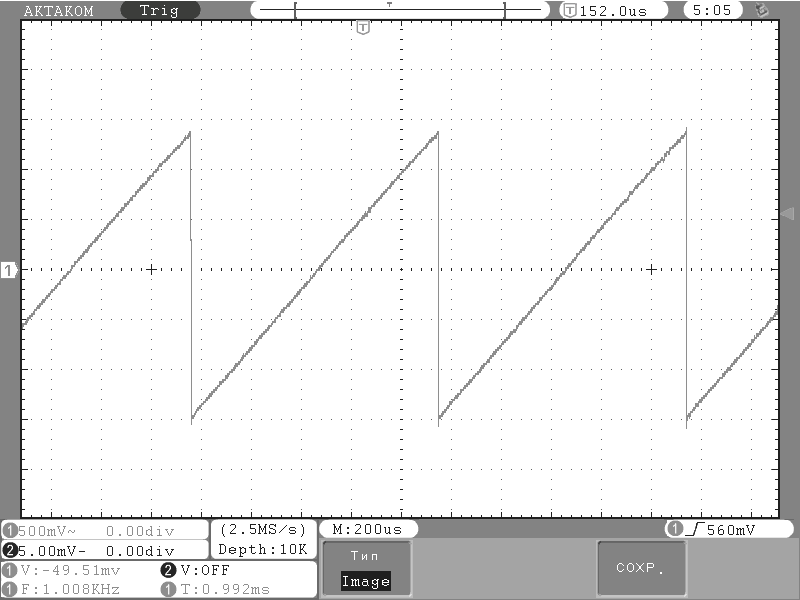
\includegraphics[width=\textwidth]{r_saw1}
         \caption*{Пилообразная}
     \end{subfigure}
     \hfill
     \begin{subfigure}[H]{0.4\textwidth}
         \centering
         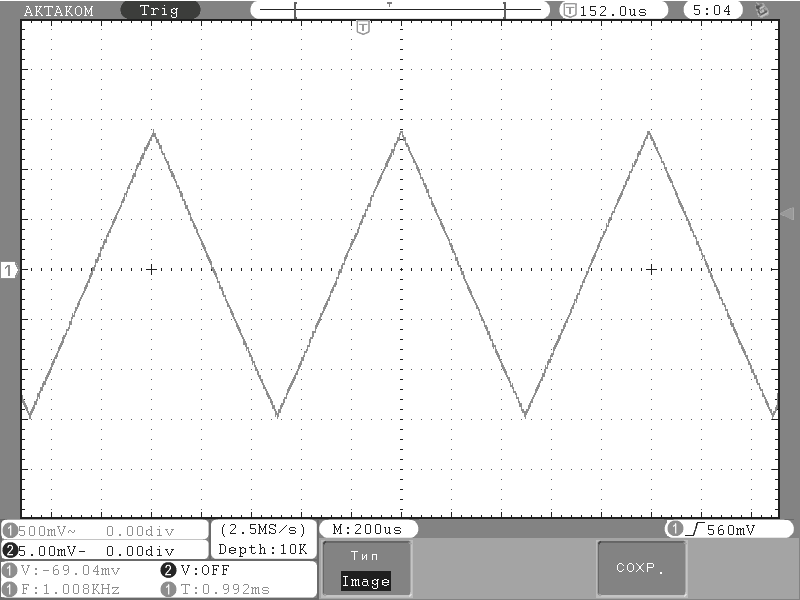
\includegraphics[width=\textwidth]{triangle1}
         \caption*{Треугольная}
     \end{subfigure}
     \hfill
     \begin{subfigure}[H]{0.4\textwidth}
         \centering
         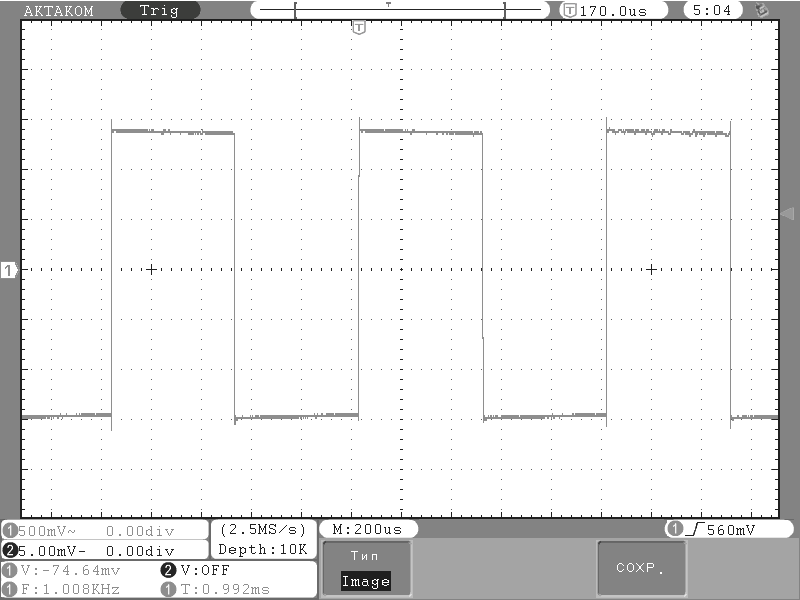
\includegraphics[width=\textwidth]{square1}
         \caption*{Прямоугольная}
     \end{subfigure}
        \caption*{Формы сигналов на частоте 1 кГц.}
\end{figure}
\end{frame}

\begin{frame}{Тестирование}
  \begin{figure}
  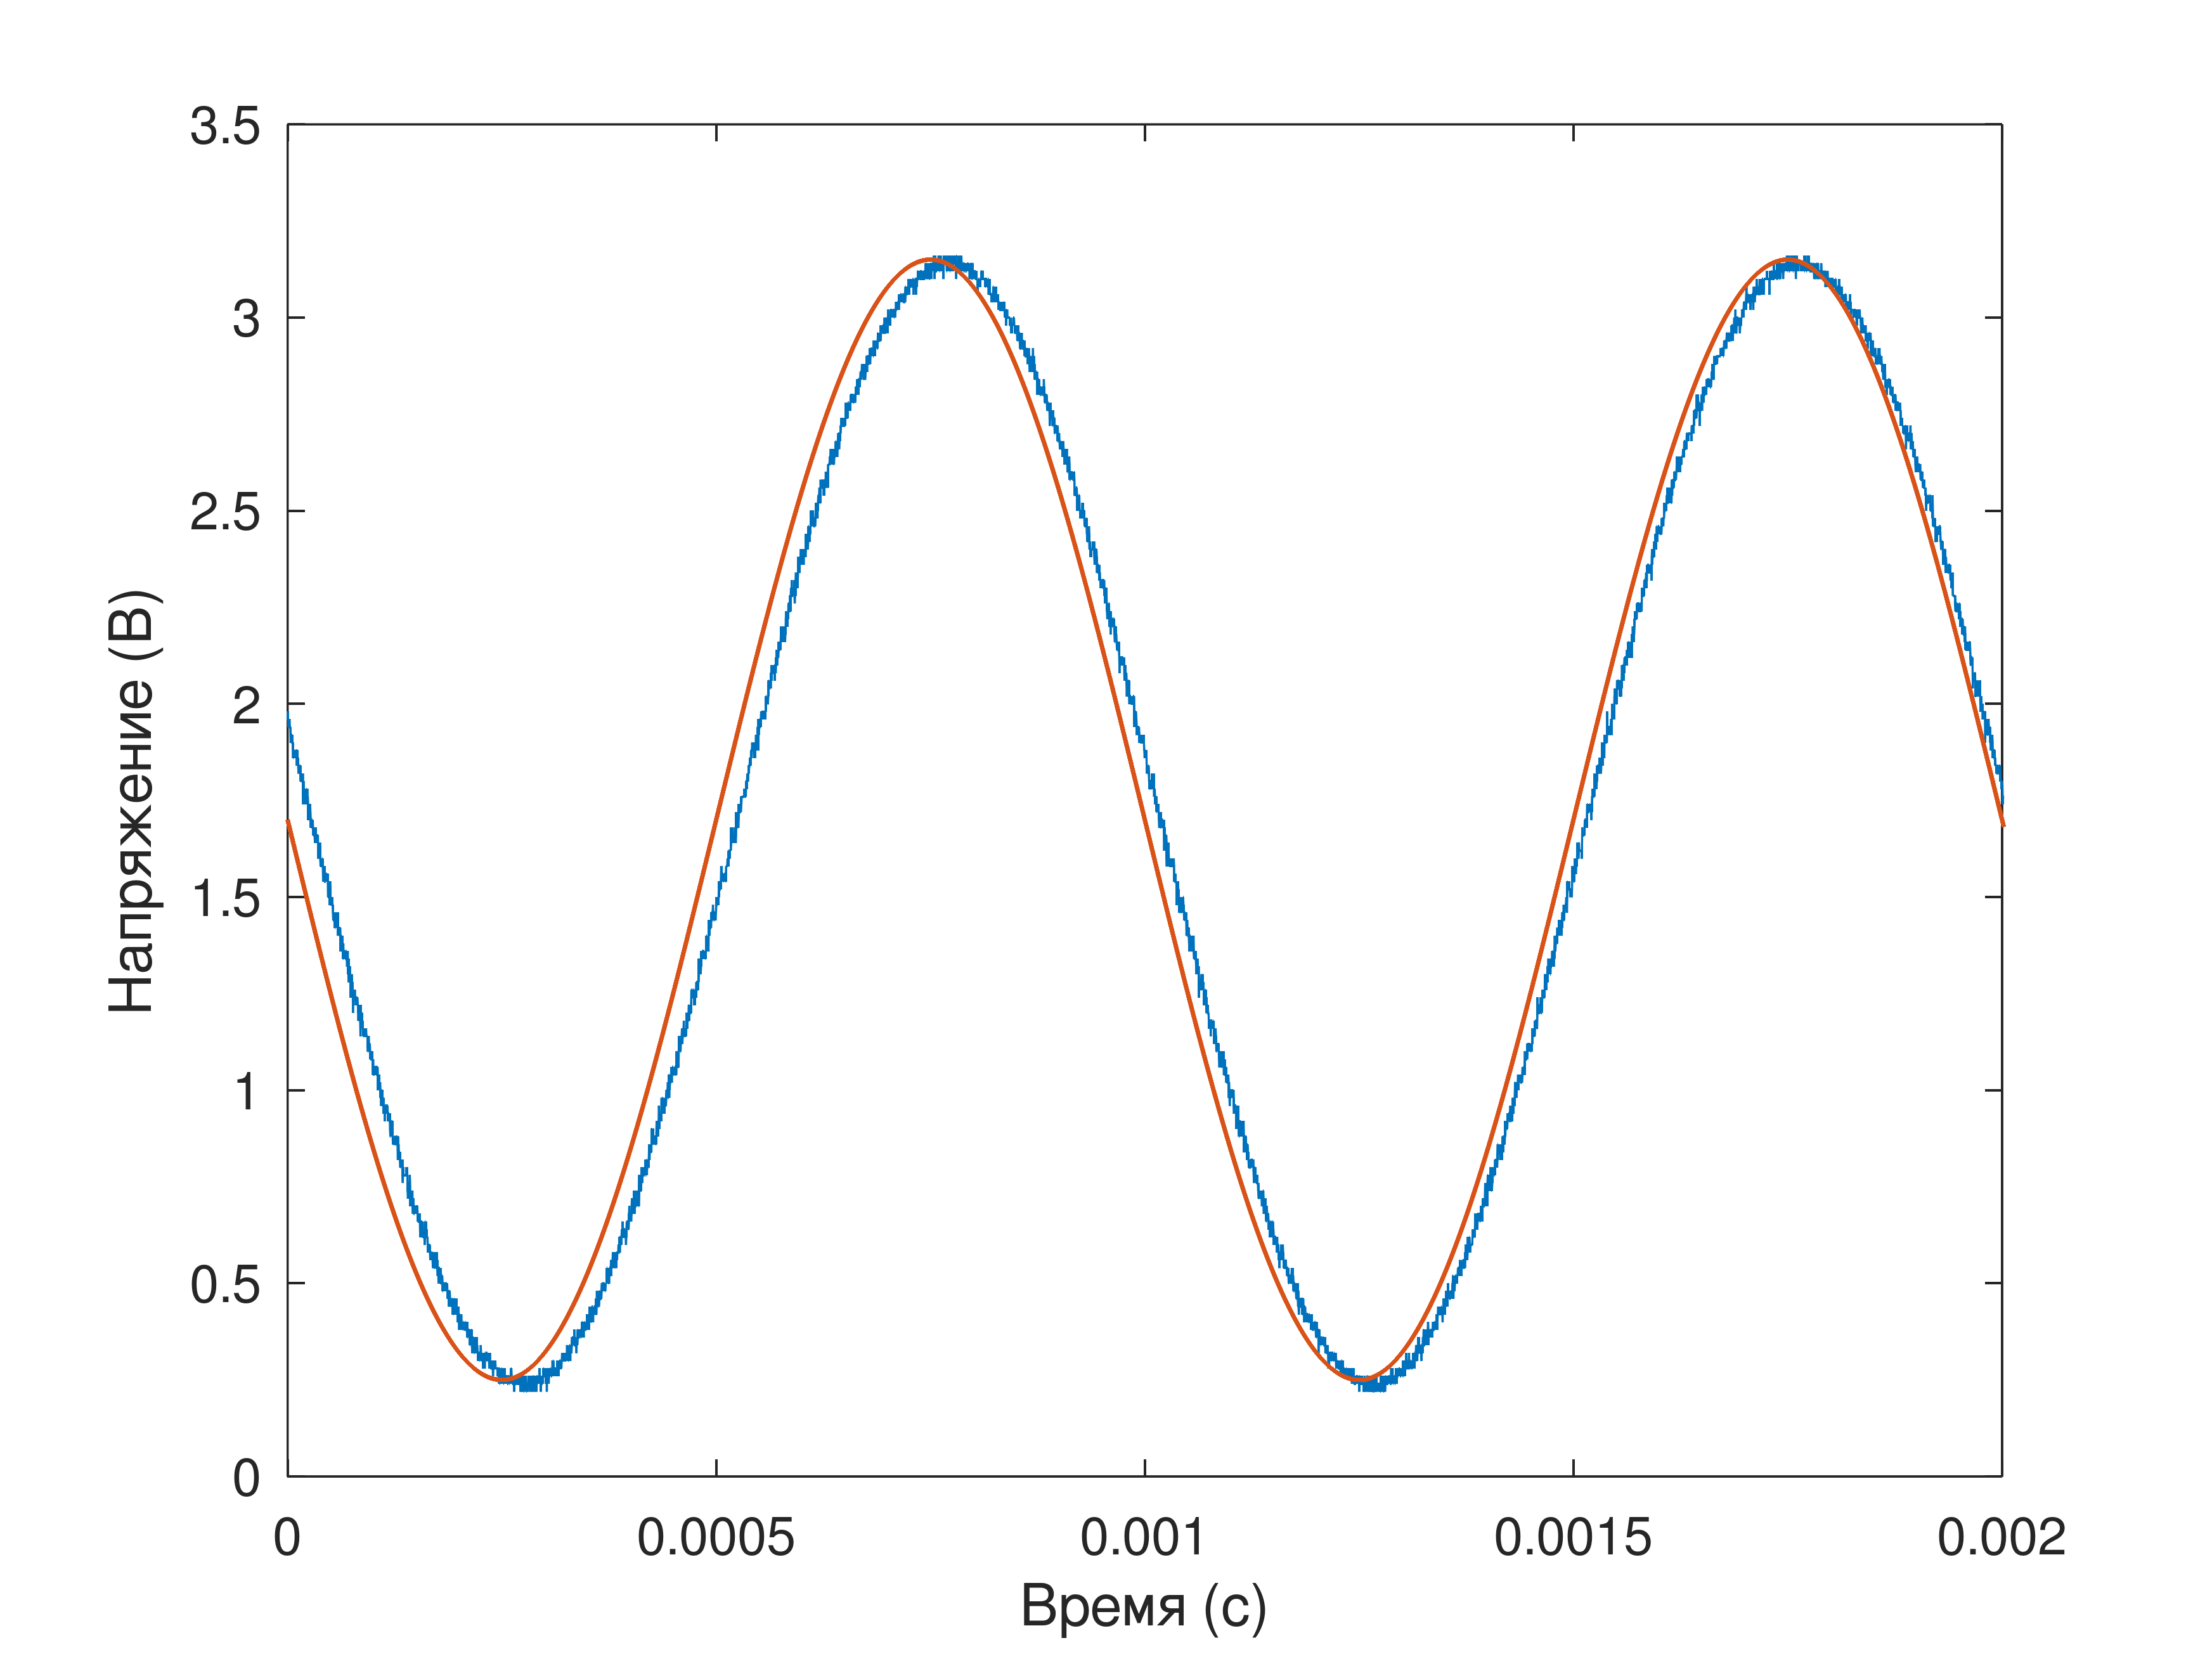
\includegraphics[width=0.95\textwidth]{test}
  \caption*{Сравнение записанного (синий) и идеального (оранжевый) сигналов.}
  \end{figure}
\end{frame}

\begin{frame}{Тестирование}
  \begin{figure}
  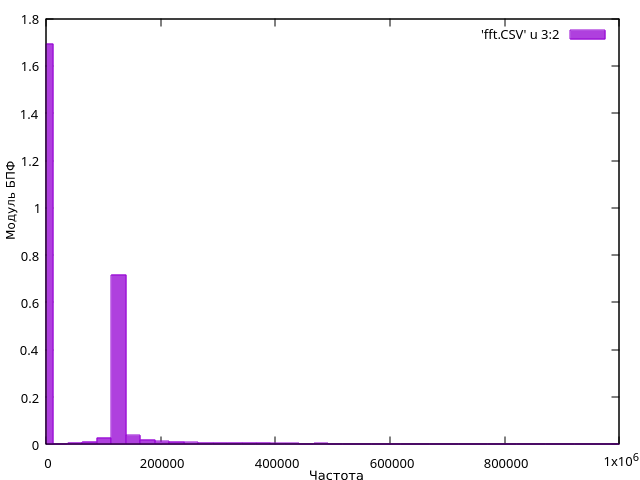
\includegraphics[width=1\textwidth]{fft}
  \caption*{Спектр сигнала.}
  \end{figure}
\end{frame}

\begin{frame}{Заключение}

	В ходе выполнения работы цель была достигнута: разработан программный генератор сигналов на микроконтроллере STM32F103RCT6, позволяющий генерировать сигналы разной формы со следующими характеристиками:
	\begin{itemize}
		\item Формы сигналов: синус, треугольник, прямоугольник, пилообразная, обратная пилообразная.
		\item Частота сигнала: 125 --- 50000 Гц.
		\item Шаг по частоте: 125, 250, 500, 1000 Гц.
	\end{itemize}

	Были выполнены все поставленные задачи, а именно:
	\begin{enumerate}
		\item Выбран метод генерации сигналов;
		\item Выбран микроконтроллер;
		\item Выбрана среда разработки;
		\item Разработана программа;
		\item Спроектировано устройство;
		\item Протестирован генератор.
	\end{enumerate}
	
	
	

\end{frame}

\begin{frame}
\begin{center}
{\Huge Спасибо за внимание! }
\end{center}
\end{frame}

\end{document}
